\begin{enumerate}[label=\thesubsection.\arabic*.,ref=\thesubsection.\theenumi]
\numberwithin{equation}{enumi}

\item Sketch the Nyquist plot for a closed loop system having open-loop transfer function 
\begin{align}
\label{eq:ee18btech11035_GH}
    G\brak{s}H\brak{s}=\frac{2e^{-s\tau}}{s\brak{1+s}\brak{1+0.5s}}
\end{align}
Determine the maximum value of $\tau$ for the system to be stable.

\item Find $\text{Re} \cbrak{G(\j\omega)H(\j\omega)}$ and $\text{Im} \cbrak{G(\j\omega)H(\j\omega)}$.\\
\solution From \eqref{eq:ee18btech11035_GH},

\begin{multline}
\label{eq:ee18btech11035_Re}
\implies  \text{Re} \cbrak{G(\j\omega)H(\j\omega)} =
\\
-4\sbrak{\frac{3\omega^2\cos\brak{\omega\tau}-\brak{\omega^3-2\omega}\sin\brak{\omega\tau}}{  \brak{3\omega^2}^2+ \brak{\omega^3-2\omega}^2  }}
\end{multline}

\begin{multline}
\label{eq:ee18btech11035_Im}
\implies  \text{Im} \cbrak{G(\j\omega)H(\j\omega)} =
\\
4\sbrak{\frac{\brak{\omega^3-2\omega}\cos\brak{\omega\tau}+3\omega^2\sin\brak{\omega\tau}}{  \brak{3\omega^2}^2+ \brak{\omega^3-2\omega}^2  }}
\end{multline}

\item Determine the maximum value of $\tau$ for the system to be stable.\\
\solution Determining the stability of closed loop transfer function using Nyquist stability Criterion.\\
\begin{align}
    Z=P+N
\end{align}
Poles of open loop transfer function are on left half of s-plane.Therefore,$P=0$\\
To ensure that the system is stable $N$ should be 0\\
For maximum value of $\tau$ for stability ,the nyquist plot cuts the real axis at -1+j0.\\
\begin{align}
    G\brak{s}H\brak{s} &= -1+j0\\
    \label{eq:ee18btech11035_im0}
    \text{Im} \cbrak{G(\j\omega)H(\j\omega)} &= 0\\
    \label{eq:ee18btech11035_Re0}
    \text{Re} \cbrak{G(\j\omega)H(\j\omega)} &= -1
\end{align}

From \eqref{eq:ee18btech11035_Im} and \eqref{eq:ee18btech11035_im0}
\begin{align}
    \label{eq:ee18btech11035_tan}
    \implies \tan\brak{\omega\tau}&=\frac{-\brak{\omega^3-2\omega}}{3\omega^2}
\end{align}

From \eqref{eq:ee18btech11035_Re} and \eqref{eq:ee18btech11035_Re0} and substituting \tan\brak{\omega\tau}&=\frac{-\brak{\omega^3-2\omega}}{3\omega^2}


\begin{align}
    \label{eq:ee18btech11035_omega}
    \implies  \omega^6+5\omega^4+4\omega^2-16=0
\end{align}

Solving \eqref{eq:ee18btech11035_omega} graphically.\\

\begin{figure}[!h]
  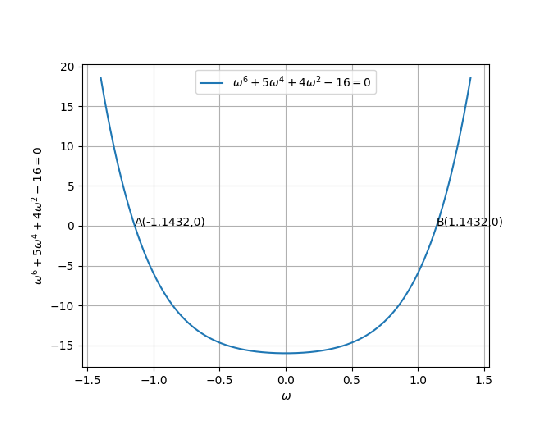
\includegraphics[width=\columnwidth]{./figs/ee18btech11035_1.eps}
  \caption{}
  \label{fig:ee18btech11035_1}
\end{figure}
Pyhton code for the above plot is
\begin{lstlisting}
codes/ee18btech11035_1.py
\end{lstlisting}

$\omega$ = 1.1432,-1.1432 \brak{As,\omega\text{ is positive}}\\
Therefore,$\omega$ = 1.1432\\

Substituting $\omega$ in \eqref{eq:ee18btech11035_tan}\\
\begin{align}
    \tan\brak{1.1432\tau}&=0.2021\\
    \tau&=0.1744
\end{align}

\item Sketch the Nyquist plot.
\\
\solution The following python code generates the Nyquist plot.
\begin{lstlisting}
codes/ee18btech11035_2.py
\end{lstlisting}

\begin{figure}[!h]
  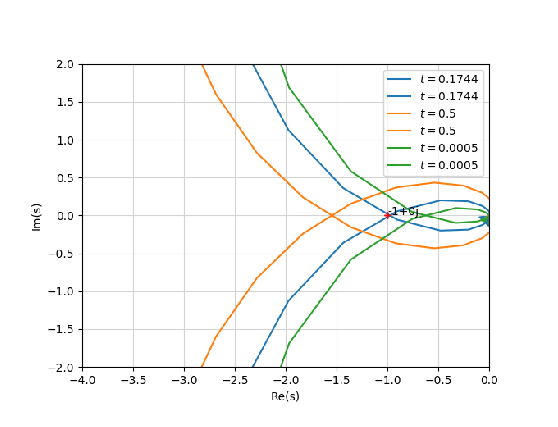
\includegraphics[width=\columnwidth]{./figs/ee18btech11035_2.eps}
  \caption{Nyquist plot for variable $\tau$}
  \label{fig:ee18btech11035_2}
\end{figure}

From the above figure \eqref{fig:ee18btech11035_2} $\tau \le 0.1744$ for a stable system.

\item Stability Criterion as varying $\tau$ 
\\
\solution 
\begin{table}[!ht]
\centering
%%%%%%%%%%%%%%%%%%%%%%%%%%%%%%%%%%%%%%%%%%%%%%%%%%%%%%%%%%%%%%%%%%%%%%
%%                                                                  %%
%%  This is the header of a LaTeX2e file exported from Gnumeric.    %%
%%                                                                  %%
%%  This file can be compiled as it stands or included in another   %%
%%  LaTeX document. The table is based on the longtable package so  %%
%%  the longtable options (headers, footers...) can be set in the   %%
%%  preamble section below (see PRAMBLE).                           %%
%%                                                                  %%
%%  To include the file in another, the following two lines must be %%
%%  in the including file:                                          %%
%%        \def\inputGnumericTable{}                                 %%
%%  at the beginning of the file and:                               %%
%%        \input{name-of-this-file.tex}                             %%
%%  where the table is to be placed. Note also that the including   %%
%%  file must use the following packages for the table to be        %%
%%  rendered correctly:                                             %%
%%    \usepackage[latin1]{inputenc}                                 %%
%%    \usepackage{color}                                            %%
%%    \usepackage{array}                                            %%
%%    \usepackage{longtable}                                        %%
%%    \usepackage{calc}                                             %%
%%    \usepackage{multirow}                                         %%
%%    \usepackage{hhline}                                           %%
%%    \usepackage{ifthen}                                           %%
%%  optionally (for landscape tables embedded in another document): %%
%%    \usepackage{lscape}                                           %%
%%                                                                  %%
%%%%%%%%%%%%%%%%%%%%%%%%%%%%%%%%%%%%%%%%%%%%%%%%%%%%%%%%%%%%%%%%%%%%%%



%%  This section checks if we are begin input into another file or  %%
%%  the file will be compiled alone. First use a macro taken from   %%
%%  the TeXbook ex 7.7 (suggestion of Han-Wen Nienhuys).            %%
\def\ifundefined#1{\expandafter\ifx\csname#1\endcsname\relax}


%%  Check for the \def token for inputed files. If it is not        %%
%%  defined, the file will be processed as a standalone and the     %%
%%  preamble will be used.                                          %%
\ifundefined{inputGnumericTable}

%%  We must be able to close or not the document at the end.        %%
	\def\gnumericTableEnd{\end{document}}


%%%%%%%%%%%%%%%%%%%%%%%%%%%%%%%%%%%%%%%%%%%%%%%%%%%%%%%%%%%%%%%%%%%%%%
%%                                                                  %%
%%  This is the PREAMBLE. Change these values to get the right      %%
%%  paper size and other niceties.                                  %%
%%                                                                  %%
%%%%%%%%%%%%%%%%%%%%%%%%%%%%%%%%%%%%%%%%%%%%%%%%%%%%%%%%%%%%%%%%%%%%%%

	\documentclass[12pt%
			  %,landscape%
                    ]{report}
       \usepackage[latin1]{inputenc}
       \usepackage{fullpage}
       \usepackage{color}
       \usepackage{array}
       \usepackage{longtable}
       \usepackage{calc}
       \usepackage{multirow}
       \usepackage{hhline}
       \usepackage{ifthen}

%%  End of the preamble for the standalone. The next section is for %%
%%  documents which are included into other LaTeX2e files.          %%
\else

%%  We are not a stand alone document. For a regular table, we will %%
%%  have no preamble and only define the closing to mean nothing.   %%
    \def\gnumericTableEnd{}

%%  If we want landscape mode in an embedded document, comment out  %%
%%  the line above and uncomment the two below. The table will      %%
%%  begin on a new page and run in landscape mode.                  %%
%       \def\gnumericTableEnd{\end{landscape}}
%       \begin{landscape}


%%  End of the else clause for this file being \input.              %%
\fi

%%%%%%%%%%%%%%%%%%%%%%%%%%%%%%%%%%%%%%%%%%%%%%%%%%%%%%%%%%%%%%%%%%%%%%
%%                                                                  %%
%%  The rest is the gnumeric table, except for the closing          %%
%%  statement. Changes below will alter the table's appearance.     %%
%%                                                                  %%
%%%%%%%%%%%%%%%%%%%%%%%%%%%%%%%%%%%%%%%%%%%%%%%%%%%%%%%%%%%%%%%%%%%%%%

\providecommand{\gnumericmathit}[1]{#1} 
%%  Uncomment the next line if you would like your numbers to be in %%
%%  italics if they are italizised in the gnumeric table.           %%
%\renewcommand{\gnumericmathit}[1]{\mathit{#1}}
\providecommand{\gnumericPB}[1]%
{\let\gnumericTemp=\\#1\let\\=\gnumericTemp\hspace{0pt}}
 \ifundefined{gnumericTableWidthDefined}
        \newlength{\gnumericTableWidth}
        \newlength{\gnumericTableWidthComplete}
        \newlength{\gnumericMultiRowLength}
        \global\def\gnumericTableWidthDefined{}
 \fi
%% The following setting protects this code from babel shorthands.  %%
 \ifthenelse{\isundefined{\languageshorthands}}{}{\languageshorthands{english}}
%%  The default table format retains the relative column widths of  %%
%%  gnumeric. They can easily be changed to c, r or l. In that case %%
%%  you may want to comment out the next line and uncomment the one %%
%%  thereafter                                                      %%
\providecommand\gnumbox{\makebox[0pt]}
%%\providecommand\gnumbox[1][]{\makebox}

%% to adjust positions in multirow situations                       %%
\setlength{\bigstrutjot}{\jot}
\setlength{\extrarowheight}{\doublerulesep}

%%  The \setlongtables command keeps column widths the same across  %%
%%  pages. Simply comment out next line for varying column widths.  %%
\setlongtables

\setlength\gnumericTableWidth{%
	25pt+%
	25pt+%
	25pt+%
	25pt+%
	50pt+%
0pt}
\def\gumericNumCols{5}
\setlength\gnumericTableWidthComplete{\gnumericTableWidth+%
         \tabcolsep*\gumericNumCols*2+\arrayrulewidth*\gumericNumCols}
\ifthenelse{\lengthtest{\gnumericTableWidthComplete > \linewidth}}%
         {\def\gnumericScale{\ratio{\linewidth-%
                        \tabcolsep*\gumericNumCols*2-%
                        \arrayrulewidth*\gumericNumCols}%
{\gnumericTableWidth}}}%
{\def\gnumericScale{1}}

%%%%%%%%%%%%%%%%%%%%%%%%%%%%%%%%%%%%%%%%%%%%%%%%%%%%%%%%%%%%%%%%%%%%%%
%%                                                                  %%
%% The following are the widths of the various columns. We are      %%
%% defining them here because then they are easier to change.       %%
%% Depending on the cell formats we may use them more than once.    %%
%%                                                                  %%
%%%%%%%%%%%%%%%%%%%%%%%%%%%%%%%%%%%%%%%%%%%%%%%%%%%%%%%%%%%%%%%%%%%%%%

\ifthenelse{\isundefined{\gnumericColA}}{\newlength{\gnumericColA}}{}\settowidth{\gnumericColA}{\begin{tabular}{@{}p{25pt*\gnumericScale}@{}}x\end{tabular}}
\ifthenelse{\isundefined{\gnumericColB}}{\newlength{\gnumericColB}}{}\settowidth{\gnumericColB}{\begin{tabular}{@{}p{25pt*\gnumericScale}@{}}x\end{tabular}}
\ifthenelse{\isundefined{\gnumericColC}}{\newlength{\gnumericColC}}{}\settowidth{\gnumericColC}{\begin{tabular}{@{}p{25pt*\gnumericScale}@{}}x\end{tabular}}
\ifthenelse{\isundefined{\gnumericColD}}{\newlength{\gnumericColD}}{}\settowidth{\gnumericColD}{\begin{tabular}{@{}p{25pt*\gnumericScale}@{}}x\end{tabular}}
\ifthenelse{\isundefined{\gnumericColE}}{\newlength{\gnumericColE}}{}\settowidth{\gnumericColE}{\begin{tabular}{@{}p{50pt*\gnumericScale}@{}}x\end{tabular}}

\begin{tabular}[c]{%
	b{\gnumericColA}%
	b{\gnumericColB}%
	b{\gnumericColC}%
	b{\gnumericColD}%
	b{\gnumericColE}%
	}

%%%%%%%%%%%%%%%%%%%%%%%%%%%%%%%%%%%%%%%%%%%%%%%%%%%%%%%%%%%%%%%%%%%%%%
%%  The longtable options. (Caption, headers... see Goosens, p.124) %%
%	\caption{The Table Caption.}             \\	%
% \hline	% Across the top of the table.
%%  The rest of these options are table rows which are placed on    %%
%%  the first, last or every page. Use \multicolumn if you want.    %%

%%  Header for the first page.                                      %%
%	\multicolumn{3}{c}{The First Header} \\ \hline 
%	\multicolumn{1}{c}{colTag}	%Column 1
%	&\multicolumn{1}{c}{colTag}	%Column 2
%	&\multicolumn{1}{c}{colTag}	\\ \hline %Last column
%	\endfirsthead

%%  The running header definition.                                  %%
%	\hline
%	\multicolumn{3}{l}{\ldots\small\slshape continued} \\ \hline
%	\multicolumn{1}{c}{colTag}	%Column 1
%	&\multicolumn{1}{c}{colTag}	%Column 2
%	&\multicolumn{1}{c}{colTag}	\\ \hline %Last column
%	\endhead

%%  The running footer definition.                                  %%
%	\hline
%	\multicolumn{3}{r}{\small\slshape continued\ldots} \\
%	\endfoot

%%  The ending footer definition.                                   %%
%	\multicolumn{3}{c}{That's all folks} \\ \hline 
%	\endlastfoot
%%%%%%%%%%%%%%%%%%%%%%%%%%%%%%%%%%%%%%%%%%%%%%%%%%%%%%%%%%%%%%%%%%%%%%

\hhline{|-|-|-|-|-}
	 \multicolumn{1}{|p{\gnumericColA}|}%
	{\gnumericPB{\centering}\textbf{\tau}}
	&\multicolumn{1}{p{\gnumericColB}|}%
	{\gnumericPB{\centering}\textbf{P}}
	&\multicolumn{1}{p{\gnumericColC}|}%
	{\gnumericPB{\centering}\textbf{N}}
	&\multicolumn{1}{p{\gnumericColD}|}%
	{\gnumericPB{\centering}\textbf{Z}}
	&\multicolumn{1}{p{\gnumericColE}|}%
	{\gnumericPB{\raggedright}\textbf{Description}}
	
\\
\hhline{|-----|}
	 \multicolumn{1}{|p{\gnumericColA}|}%
	{\gnumericPB{\centering}{0.1744}}
	&\multicolumn{1}{p{\gnumericColB}|}%
	{\gnumericPB{\centering}0}
	&\multicolumn{1}{p{\gnumericColC}|}%
	{\gnumericPB{\centering}1}
	&\multicolumn{1}{p{\gnumericColD}|}%
	{\gnumericPB{\centering}1}
	&\multicolumn{1}{p{\gnumericColE}|}%
	{\gnumericPB{\raggedright}System is unstable}
\\
\hhline{|-----|}
	 \multicolumn{1}{|p{\gnumericColA}|}%
	{\gnumericPB{\centering}0.5}
	&\multicolumn{1}{p{\gnumericColB}|}%
	{\gnumericPB{\centering}0}
	&\multicolumn{1}{p{\gnumericColC}|}%
	{\gnumericPB{\centering}0}
	&\multicolumn{1}{p{\gnumericColD}|}%
	{\gnumericPB{\centering}0}
	&\multicolumn{1}{p{\gnumericColE}|}%
	{\gnumericPB{\raggedright}System is marginally stable}
\\

\hhline{|-|-|-|-|-|}
    \multicolumn{1}{|p{\gnumericColA}|}%
	{\gnumericPB{\centering}0.0005}
	&\multicolumn{1}{p{\gnumericColB}|}%
	{\gnumericPB{\centering}0}
	&\multicolumn{1}{p{\gnumericColC}|}%
	{\gnumericPB{\centering}0}
	&\multicolumn{1}{p{\gnumericColD}|}%
	{\gnumericPB{\centering}0}
	&\multicolumn{1}{p{\gnumericColE}|}%
	{\gnumericPB{\raggedright}System is stable}
\\
\hhline{|-|-|-|-|-|}
\end{tabular}

\ifthenelse{\isundefined{\languageshorthands}}{}{\languageshorthands{\languagename}}
\gnumericTableEnd

\caption{}
\label{table:ee18btech11035_table}
\end{table}

Therefore,$\tau_{max} = 0.1744 $\\.
\end{enumerate}
